\documentclass[a4paper, 10pt, conference]{ieeeconf}    

\usepackage{caption, graphicx, amsmath, tabularx, indentfirst, lastpage, dsfont}    
\usepackage{fancyhdr}
\pagestyle{fancy}
\fancyhf{}
\renewcommand{\headrulewidth}{0.4pt}
\renewcommand{\footrulewidth}{0.4pt}
\cfoot{\thepage\ of 5}                                   
                                                       
\IEEEoverridecommandlockouts
\overrideIEEEmargins
\usepackage{float}
\floatstyle{ruled}
\restylefloat{figure}  
\restylefloat{table}    
\title{\Large \bf
Investigating the Relationship between \\ Drugs and Criminal Behaviors / Emotional Stress \\ using Propensity Score Matching, an Observational Study}
\author{Darshan Patel}

\begin{document}
\maketitle
\thispagestyle{fancy}
\begin{abstract}

To understand the association between smoking cigarette and marijuana and criminal behaviors and emotional stress indicators. The criminal acts studied here are theft, arson and burglary. Signs of emotional stress that were studied include nervousness, hopelessness and worthlessness. It was found that smoking cigarette and criminal behavior were related, as well as smoking marijuana and emotional stress indicators. 
\end{abstract}

\section{INTRODUCTION}

The use of drugs is a public health problem all over the world. This is of interest for two reasons. One is, the rise of criminal behaviors when indulging in drugs. whereas the other is the indication of mental stress. 

Common crimes that get committed include motor vehicle theft, burglary, arson, DUI, sexual offense, fraud and other violent offenses. There are several factors that can indicate why people undergo these criminal behaviors. From having relationship issues, to financial problems, or feeling of insecurity, people over time have committed crimes to get what they want. An underlying reasoning can also be whether they were in the influence of drugs. For instance, DUI is abbreviation for driving under influence; one can only get committed for this when definitely under the influence of alcohol and drugs. But a more subtle relationship can be dug for other crimes. 

Apart from committing crimes, people often take drugs when they were not feeling good mentally. When one is feeling down due to family problems, school pressure or financial issues, they look to drugs to take away the stress for a temporary amount of time. For instance, in high school, many students enjoy smoking marijuana during school hours to relieve themselves. Signs of mental stress include anxiety, isolation, moodiness, unhappiness and more. 

In this paper, several criminal offenses and mental stress indicators will be studied. The crimes that are looked at theft, arson and burglary. Emotional stress indicators that are looked at are feelings of nervousness, hopelessness and worthlessness. An observational study will be done comparing the use of cigarette and marijuana in 2017 to determine whether taking drugs is indicative of someone having committed a crime or having an indication of emotional stress.


\section{Data}

The data provided for this study will come from the National Survey of Drug Use and Health, done in 2017. In the study, the purpose of the survey was to measure the prevalence of drugs in the United State and find relevant information about users and non-users. The target subject for the survey is the civilian, non-institutionalized population of the United States, who are older than 12 years at the time of the survey. The survey was done using CAI methods as well as holding minimum sample sizes per state. Demographic subgroup estimates were also made due to the large sample sizes. In the year of the study, $56, 276$ subjects were interviewed. Furthermore, drugs focused on include tobacco, marijuana, crack, cocaine, hallucinogens, heroin, inhalants, methamphetamine, pain relievers, tranquilizers, stimulants and sedatives. Various information about each drug were collected, such as whether the subject has ever taken them and if so, what age did they first try it, time since they last did it, the frequency of use in the past week, month and year, and more. For specialization, information about different strands of drugs were also noted if the drug label was big. For instance, hallucinogens was broken down into LSD, PCP, mescaline and more. Apart from drug usages, information on peoples' social environment, youth experiences, mental health, depression, consumption of alcohol, substance dependence and abuse, criminal acts, and drug treatment was also surveyed. A total of more than $2,500$ variables of information was collected or derived from survey participants. 

To aid this study, and optimize computational performance, a handful of variables were extracted. The drugs that was focused on are cigarette, a form of tobacco, and marijuana. Only if a subject has or has not taken the drug in their lifetime was of concern; meaning, there was surety in the drug usage. In Table I, the the number of smokers and non-smokers for both cigarette and marijuana is shown. 

% latex table generated in R 3.4.3 by xtable 1.8-3 package
% Wed Apr 17 15:42:07 2019
\begin{table}[ht]
\centering
\begin{tabular}{rlrr}
  \hline
 & Yes/No & Cigarette & Marijuana \\ 
  \hline
1 & No & 28971 & 32031 \\ 
  2 & Yes & 27305 & 24214 \\ 
   \hline
\end{tabular}
\caption{Usage of Cigarette and Marijuana}
\end{table}


\parindent 10pt From here on outwards, the control group is the group of subjects that don't smoke the drug whereas the treatment group is the group of subjects that do indulge in the drug. It can be seen that there are slightly more non-cigarette smokers than actual cigarette smokers. The difference for marijuana usage is more profound; there are nearly one-third more non-marijuana smokers than actual marijuana smokers. To study criminal offenses, a combination of three variables will be focused on: whether a subject has been arrested and booked for theft in the past $12$ months, and likewise for arson and burglary. To reduce the number of propensity score models to make, an indication variable will be created that represents all three of these crimes. If an individual has committed one or more of these three crimes, their value will be $1$, otherwise $0$, indicating no criminal behavior. The same technique will be utilized for the emotional stress indicators. The ones that are looked at in this study are: nervousness, hopelessness and worthlessness. If an individual has felt one (or more) of these feelings heavily during a particular month in 2017, their value will be $1$, otherwise $0$. 

Since this is an observational study and propensity score matching will be leveraged, a few covariates, or demographic information will be needed. The demographic information that was used in this study are gender, age, race and employment status. A percentage distribution of these demographics features for cigarette users is shown in Fig. 1. 
\begin{figure} 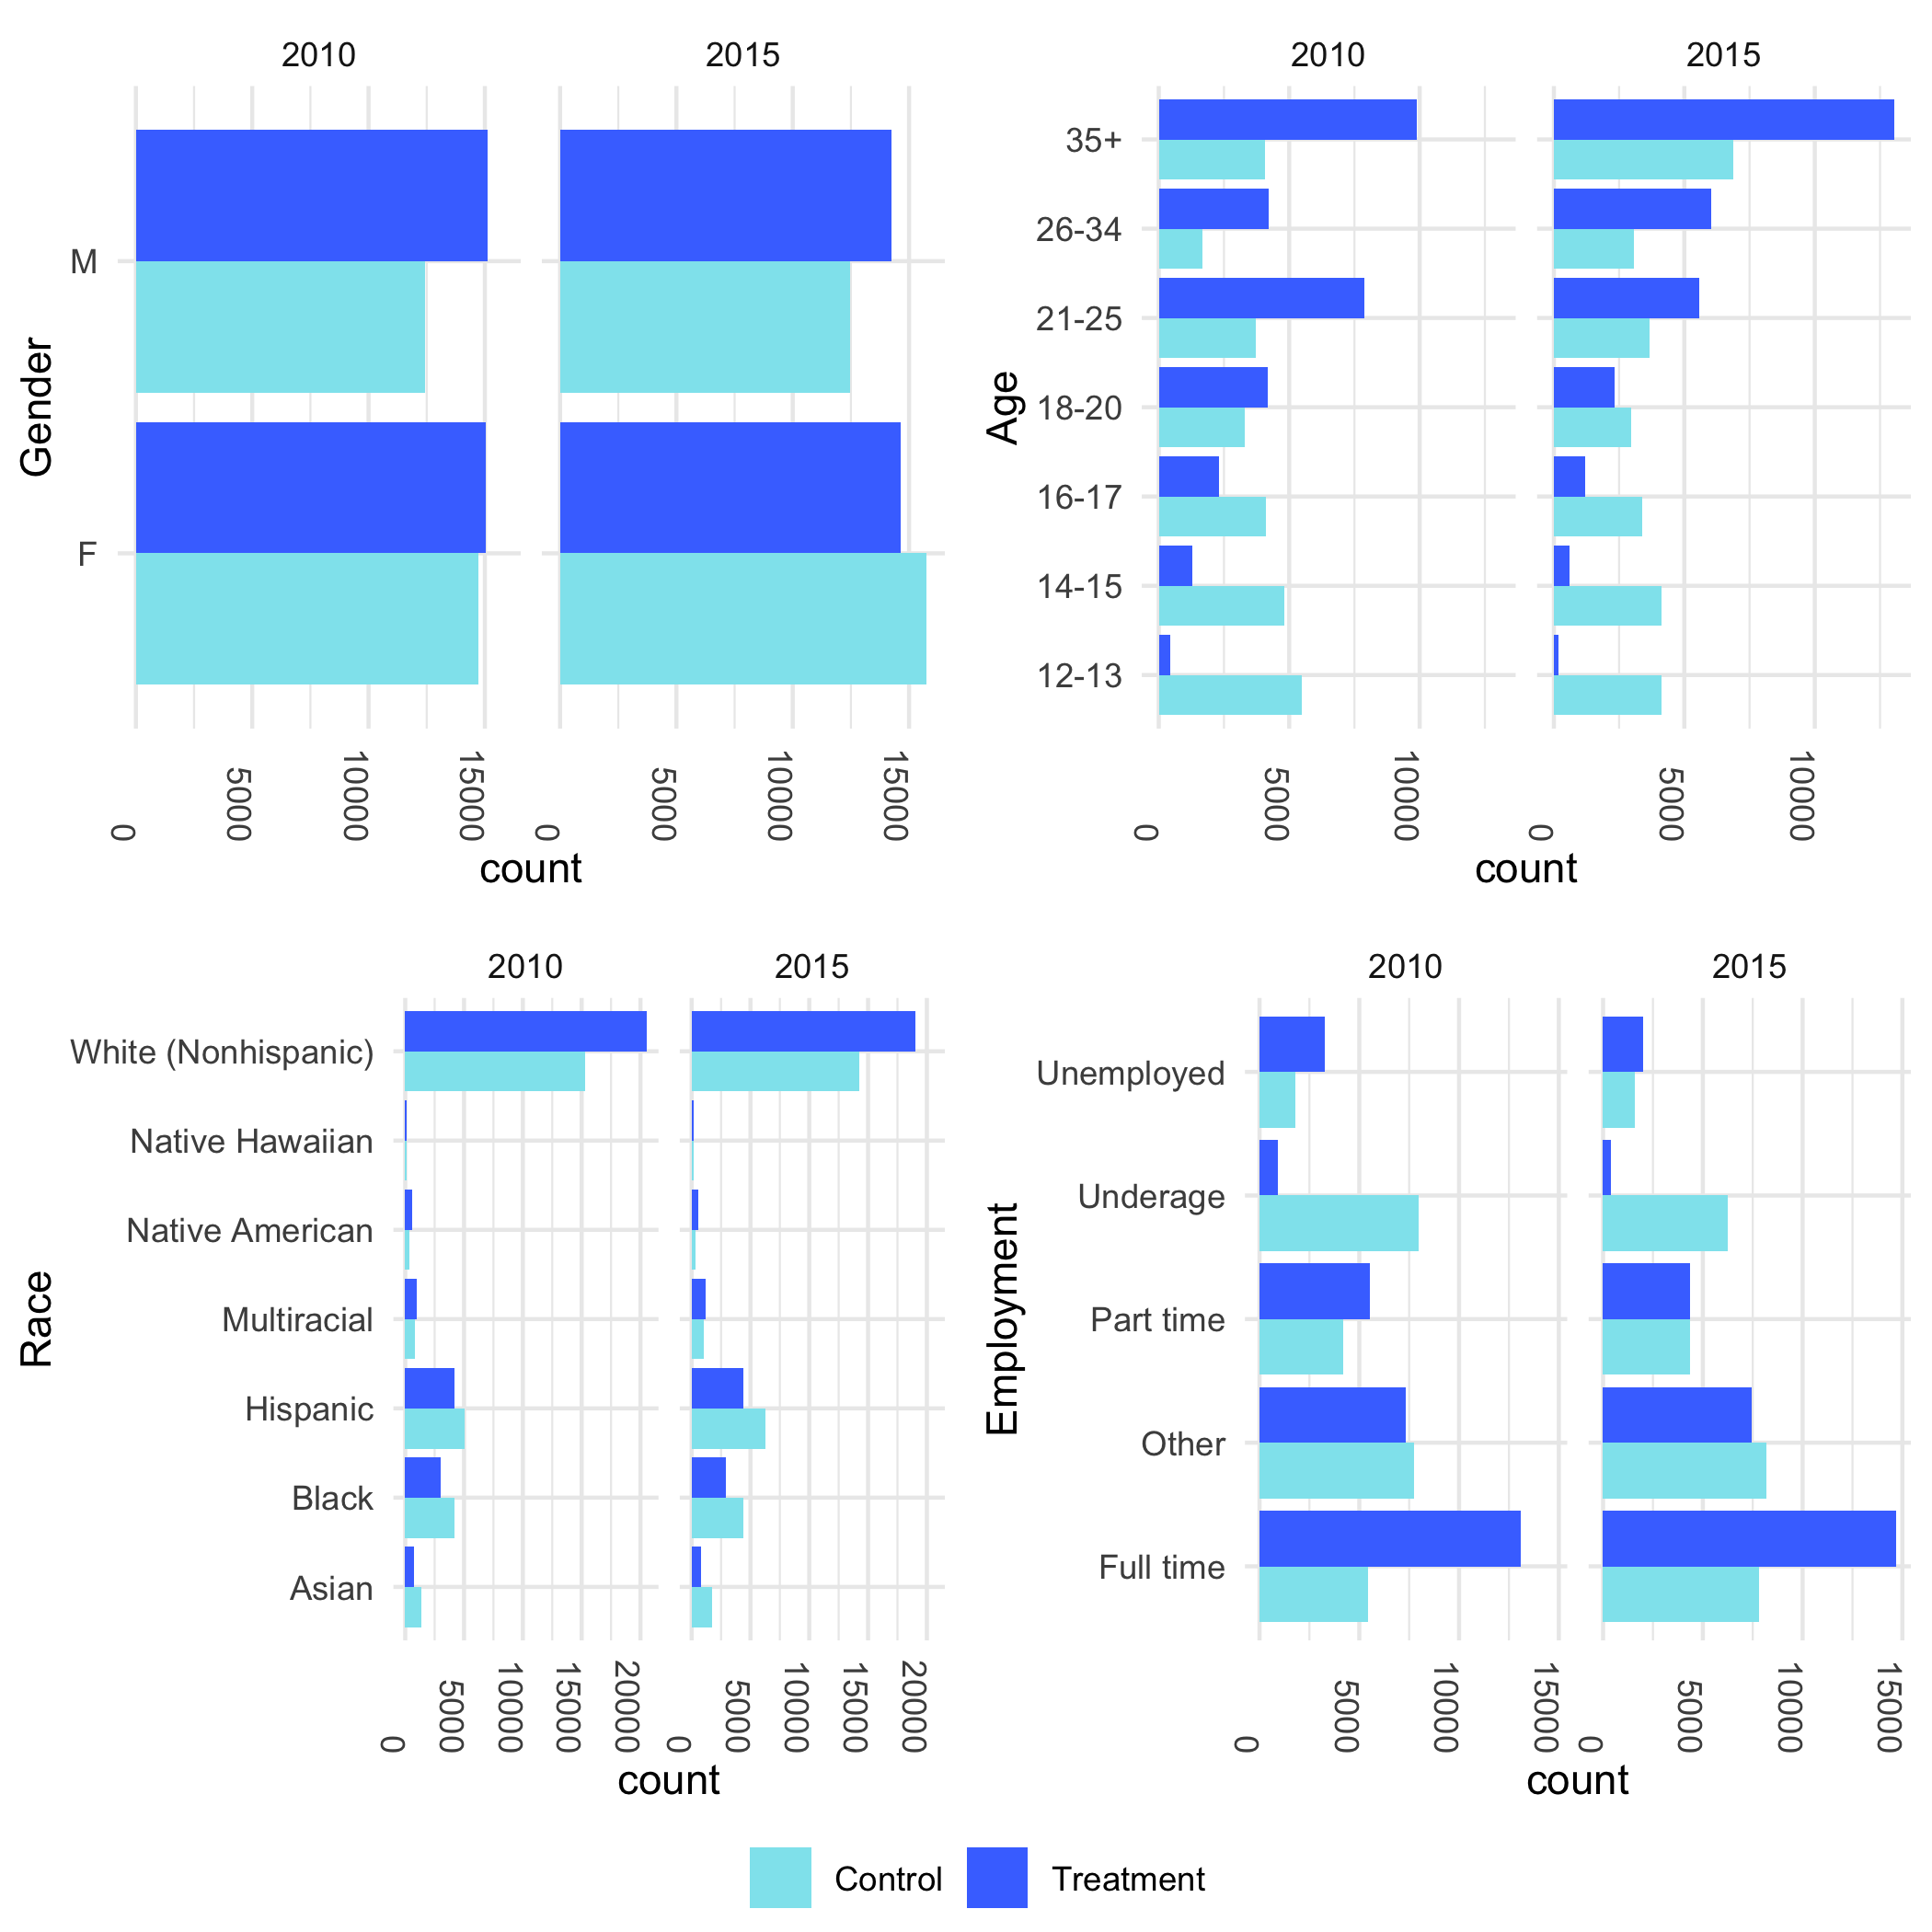
\includegraphics[scale = 0.11]{CigaretteDemographics} \captionof{figure}{Demographic Breakdown of Cigarette \\ } \end{figure} 
\parindent 10pt In this plot, the control group is the subjects who did not smoke cigarette, while the treatment group is the subjects who did. There are several takeaways from this analysis. 
First, the percentage of men and women who smoked cigarette is nearly the same. This contrasts with the fact that there are less male non-smokers than female non-smokers. Looking at the age percentage distribution, the $35+$ age group holds most of the population. As age increases, there is a growth in the percentage of cigarette users in the study while non-smokers decreases slighly until a jump at $35+$ years old. There is a huge imbalance in racial demographics in this study, where non-hispanic whites make up more than $50\%$ of the study, leaning more heavily on the cigarette user side. Lastly, it is noted that that this study there are more cigarette users who are full-time workers than those who do not; an entire $25+\%$ of the study is made up of full-time employees who smoke cigarette. This contrasts with the other employment status where percentage of non-smokers exceeds percentage of smokers. What is interesting is that unemployed people make up the lowest proportion of the study and yet have equal percentage on both sides. 

A similar analysis can be done for marijuana smokers. 
\begin{figure} 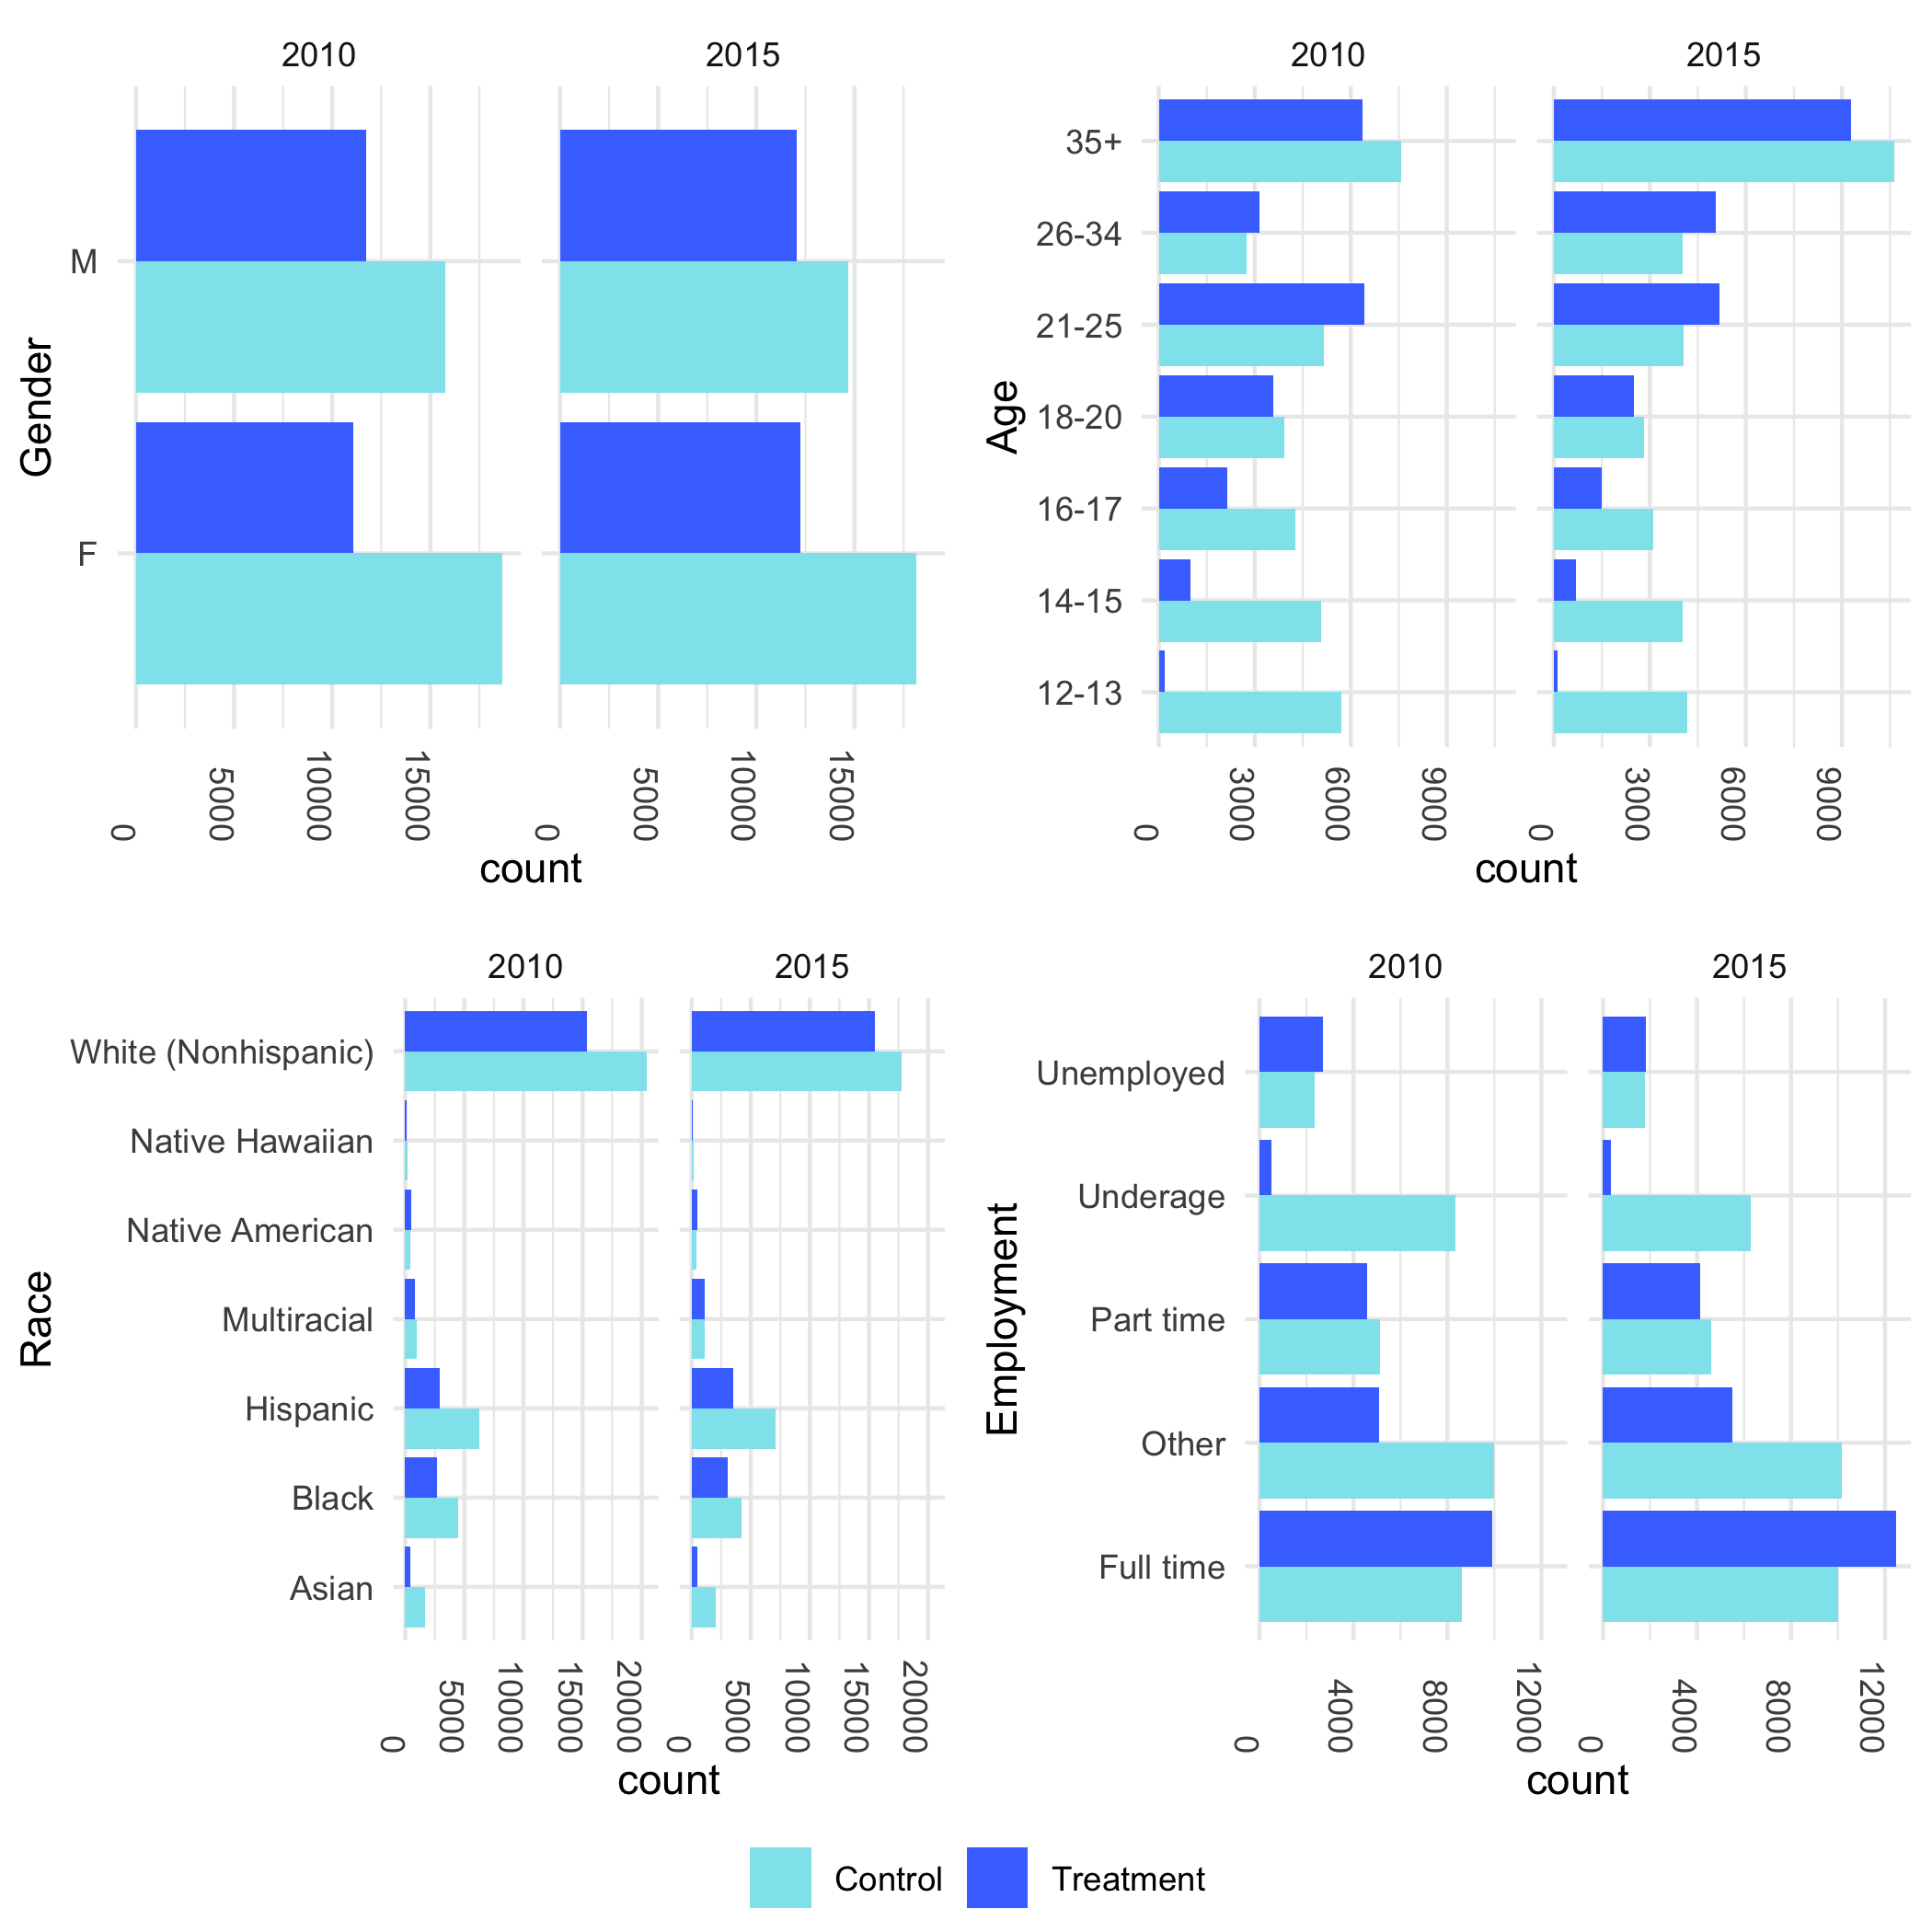
\includegraphics[scale = 0.11]{MarijuanaDemographics} \captionof{figure}{Demographic Breakdown of Marijuana \\ } \end{figure} 
\parindent 10pt A breakdown of the demographics features for marijuana use is shown in Fig. 2. The control group refers to people who have not smoked marijuana whereas the treatment group refers to people who have smoked marijuana. It is seen here that there are equally $\approx 20\%$ of marijuana smokers who are male and $\approx 20\%$ that are female. The other $60\%$ is distributed unevenly non-smokers of both genders. As for age, almost $40\%$ of the participants are $35$ years or older. In addition, the percentage of marijuana smokers and non-marijuana smokers is almost identical in that age group. In fact, the percentage for $26$ to $34$ between both groups is nearly equal as well. A total of three age groups appears to have similar distribution in groups. Looking at race, the white demographic continues to be the majority group, making up half of the population. However in this case, the non-marijuana smoker group is slightly larger than the marijuana smoker group. The number of hispanic and black people make up twice as much in the population of non-smokers than in the population of smokers. Late but not the least, there is nearly an equal distribution between the full time smokers and full time non-smokers, and likewise for part time workers. 

\section{Methods} 
\parindent 10pt After setting up the indicator variables and analyzing the data, the propensity score models were ready to be made. A total of $4$ models were made in the following manner. First, logistic regression is used to fit a propensity score model where the usage of drug is predicted using the covariates and either the crime indicator or stress indicator. Afterwards, the propensity score distance matrix was built. Using this matrix, the propensity scores from the model were matched pair-wise to form pairs of observations with differing response variable. Using these matched pairs only, a new logistic regression model was built to predict an indication of crime or stress using the covariates and drug. Lastly, the estimate for the drug coefficient in the logistic regression model was used to assess the impact of the drug on the response. This process was done $4$ times: to predict crime behavior for cigarette smokers and for marijuana smokers, and to predict emotional stress indication for cigarette smokers and for marijuana smokers. 

\section{Results}
In Table 2, a summary of each model is provided: the coefficient of estimate, the number of matched pairs and unmatched pairs, the $p$-value associated with the coefficient estimate and the interpretation of the estimate. The interpretation of the coefficient of estimate was derived as follows. Suppose a logistic model is created as $$ \log \left( \frac{\pi}{1-\pi} \right) = \beta_0 + \beta_1x_1 + \dots + \beta_px_p $$ where $\pi = \mathds{P}(y = 1)$ and $\log \left( \frac{\pi}{1-\pi} \right)$ is the log odds. Then $\hat{\beta}_j$, where $j > 0$, is the change in log-odds for every one unit increase in $x_j$ holding all other $x$'s fixed. A meaningful interpretation is formed by $$ (e^{\hat{\beta}_j} - 1) \times 100\%$$ which is the percentage change in odds $\frac{\pi}{1-\pi}$ for every unit increase in $x_j$ holding all other $x$'s fixed. This formula was used to find the interpretations of the coefficients in the logistic models above. % latex table generated in R 3.4.3 by xtable 1.8-3 package
% Wed Apr 17 15:44:19 2019
\begin{table}[ht]
\centering
\begin{tabular}{rlrrrrr}
  \hline
 & \small Model & $\beta$ & $n_{\text{m}}$ & $n_{\text{nm}}$ & $p$ & \small Interpretation \\ 
  \hline
1 & Cig/C & 0.18 & 124 &  62 & 0.68 & 19.96 \\ 
  2 & Mar/C & -0.58 &  85 & 140 & 0.27 & -44.29 \\ 
  3 & Cig/ES & 0.12 & 284 & 1264 & 0.33 & 13.31 \\ 
  4 & Mar/ES & 0.50 & 1308 & 196 & 0.00 & 65.20 \\ 
   \hline
\end{tabular}
\caption{Propensity Score Matches, Logistic Regression Model Coefficient and Interpretation} 
\end{table}
 

A number of observations are made about criminal behavior. In 2017, keeping all covariates constant, if an individual smokes cigarette, he/she has a $0.18$ change in the logit. In other terms, he/she has an increased percentage change in odds of $19.96\%$ of committing one of three crimes: burglary, arson or theft when all other variables are kept constant. This contrasts with the case for marijuana. A person who smokes marijuana, leaving all demographics information constant, has a decreased percentage change of $44.29\%$ of committing the crimes. This indicates that marijuana smokers are less likely to commit burglary, arson or theft crimes than non-smokers. For these two models, $124$ and $85$ matches were made. It is for the stress indicators where results go mayhem. With a change in log odds of $0.12$, a person who smokes cigarette has an increased percentage change in odds of $13.31\%$ of either having felt high levels of nervousness, hopelessness or worthlessness, when leaving all other variables constant. Furthermore, a person who smokes marijuana has an increased percentage change in odds of $65.20\%$ of having these heavy feelings, when leaving these other variables constant. This last percentage change in odds is a huge increase in probability. 

In addition to the coefficient estimates and interpretations, the distribution of the covariates after matching is helpful to look at. For the model looking at cigarette usage and criminal behaviors, the percentage distribution of the covariates is shown above in Fig. 3. 
\begin{figure}[t!] 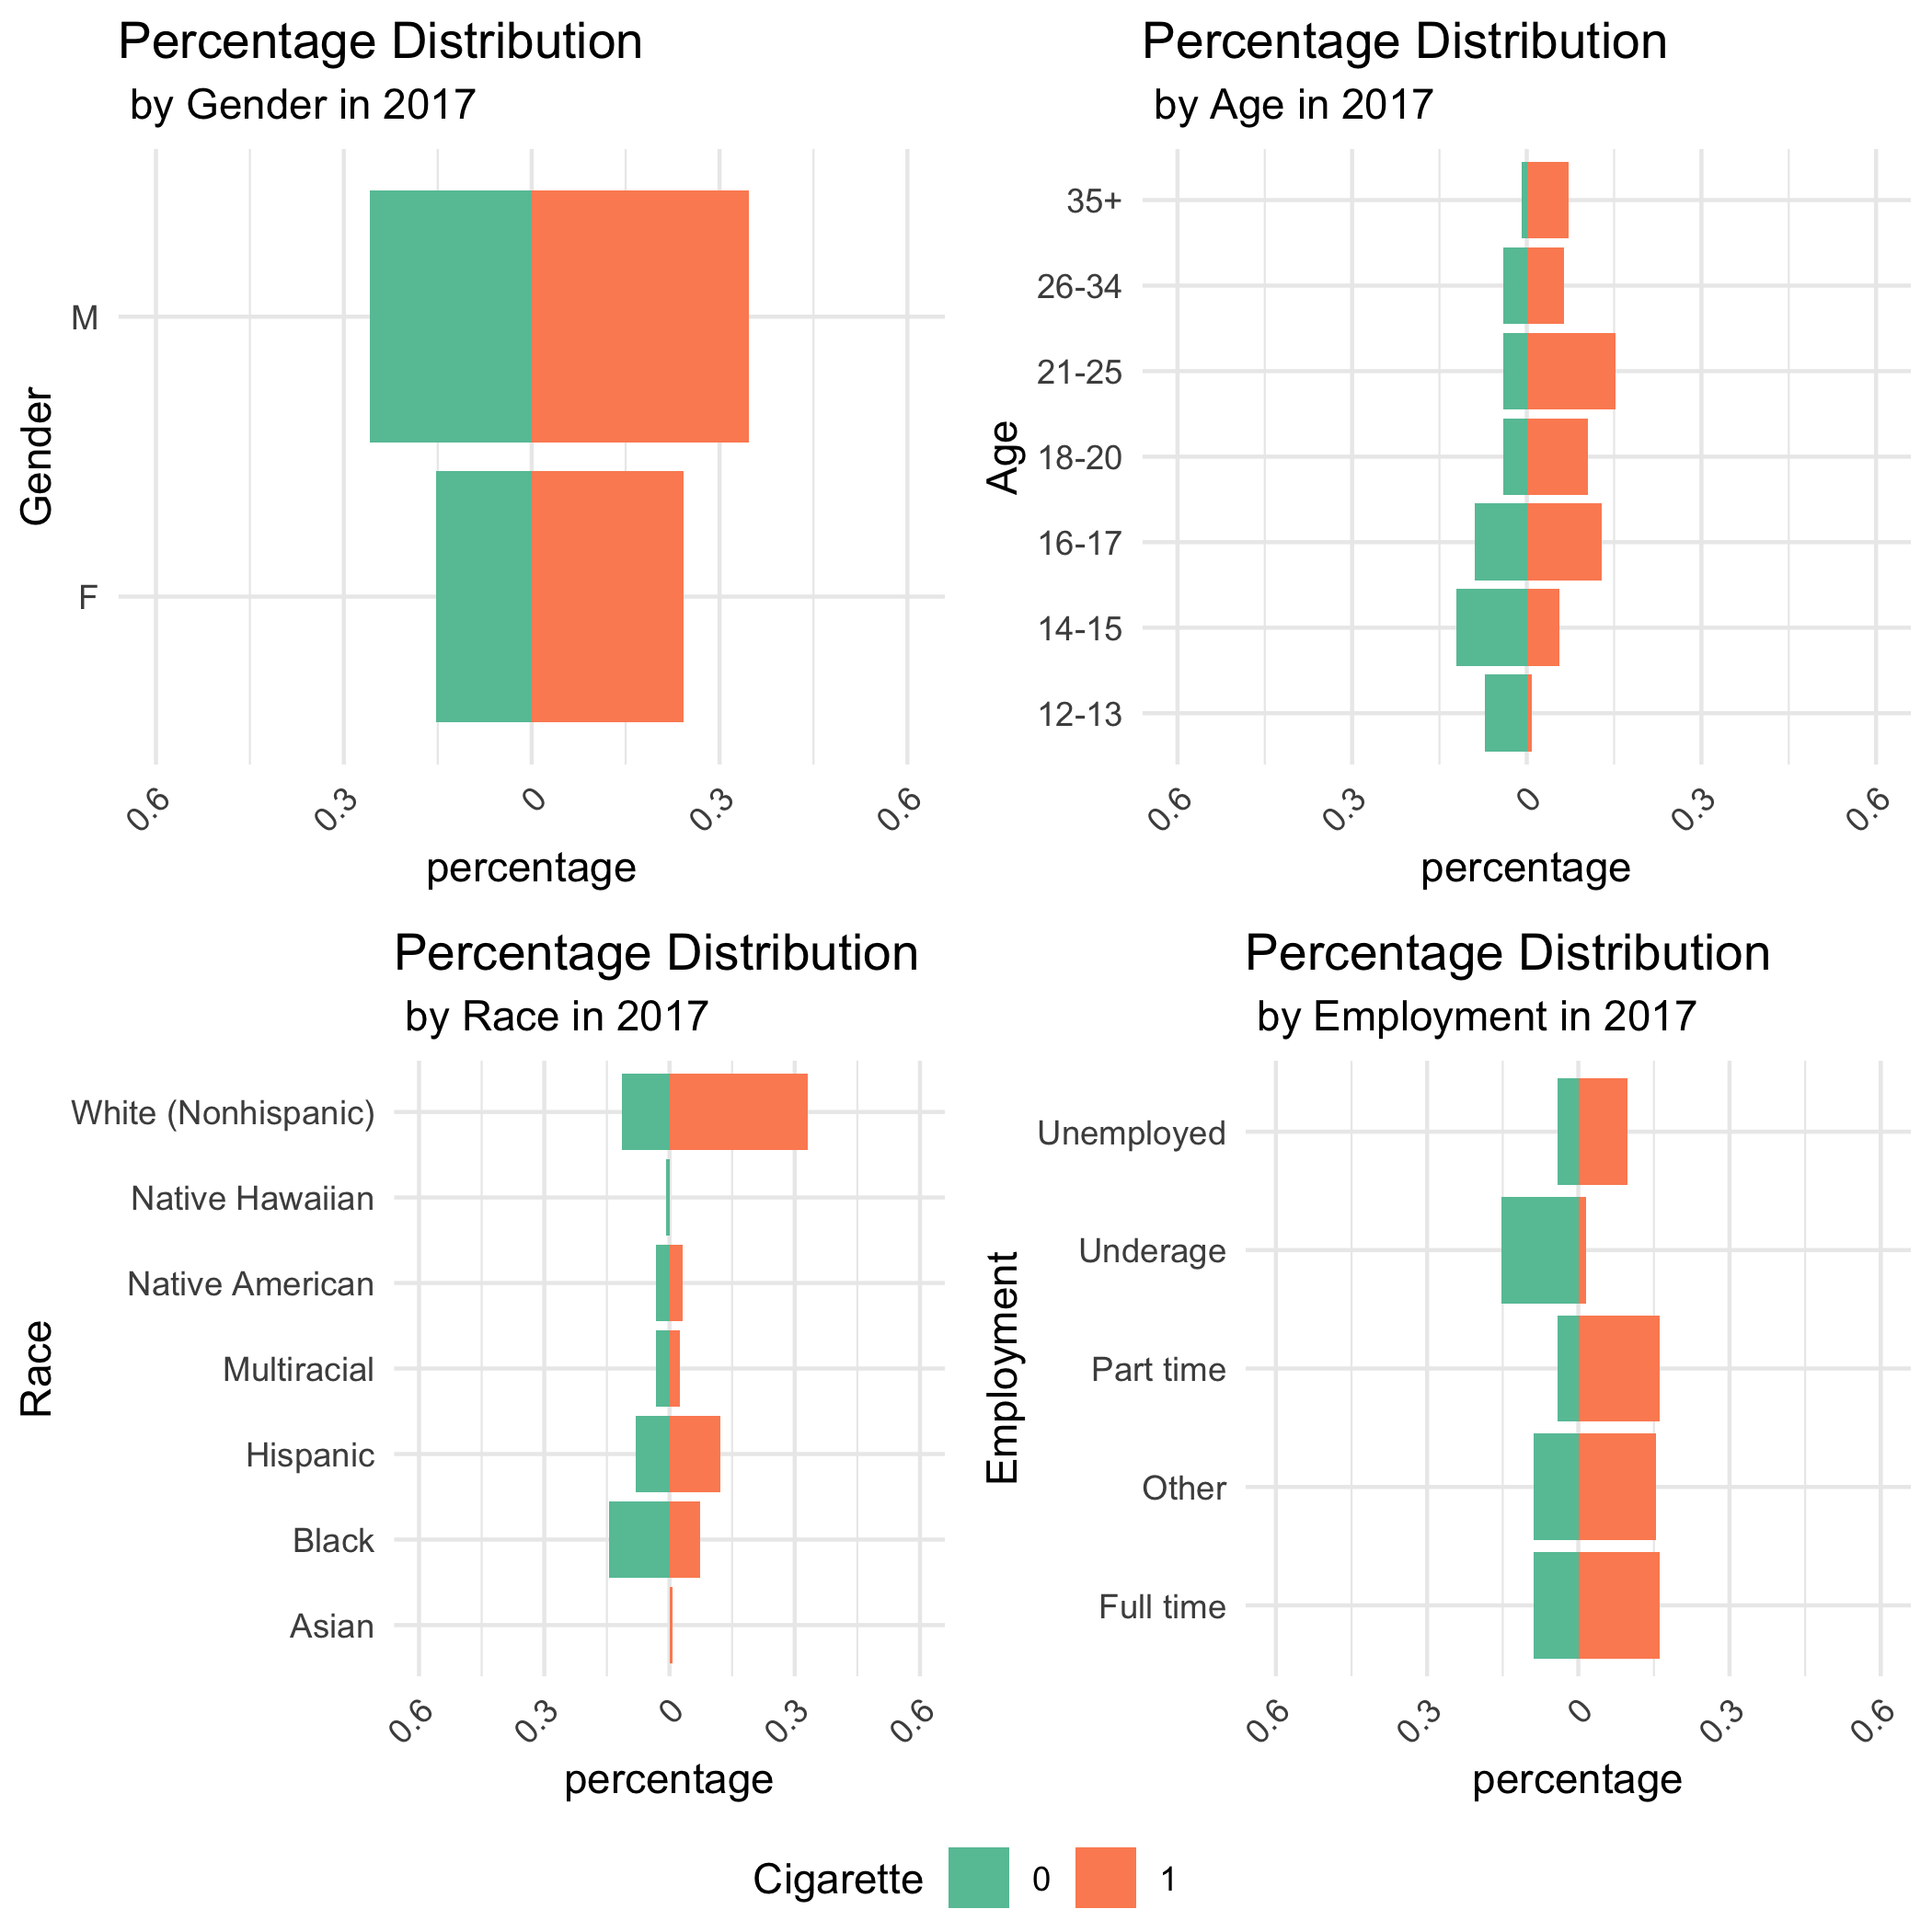
\includegraphics[scale = 0.09]{model1} \captionof{figure}{Covariate Distribution after Matching for Model 1} \end{figure}
These distributions are compared with Fig. 1 for cigarette above. What is apparent now is that gender appears to be more balanced now amongst cigarette smokers and non-cigarette smokers. It is not fully balanced in terms of proportionality though, there are more smokers than non-smokers but both genders. With the age percentage distribution, the huge imbalanced caused by the $35+$ age group is now a smaller chunk of the sample of matched sets. What appears to be in equal amounts before matching is not anymore; the percentage of white people in the sample is imbalanced. The hispanic group however does seem more balanced than before between the control and treatment group. The imbalance of full time works is reduced by the propensity score matching. Overall, some covariates have been made somewhat more balanced being the two groups but perfect balance does not exist. 

The percentage distribution of the matched covariates for the model using marijuana smokers to predict criminal behaviors is shown below in Fig. 4. \begin{figure}[t!] 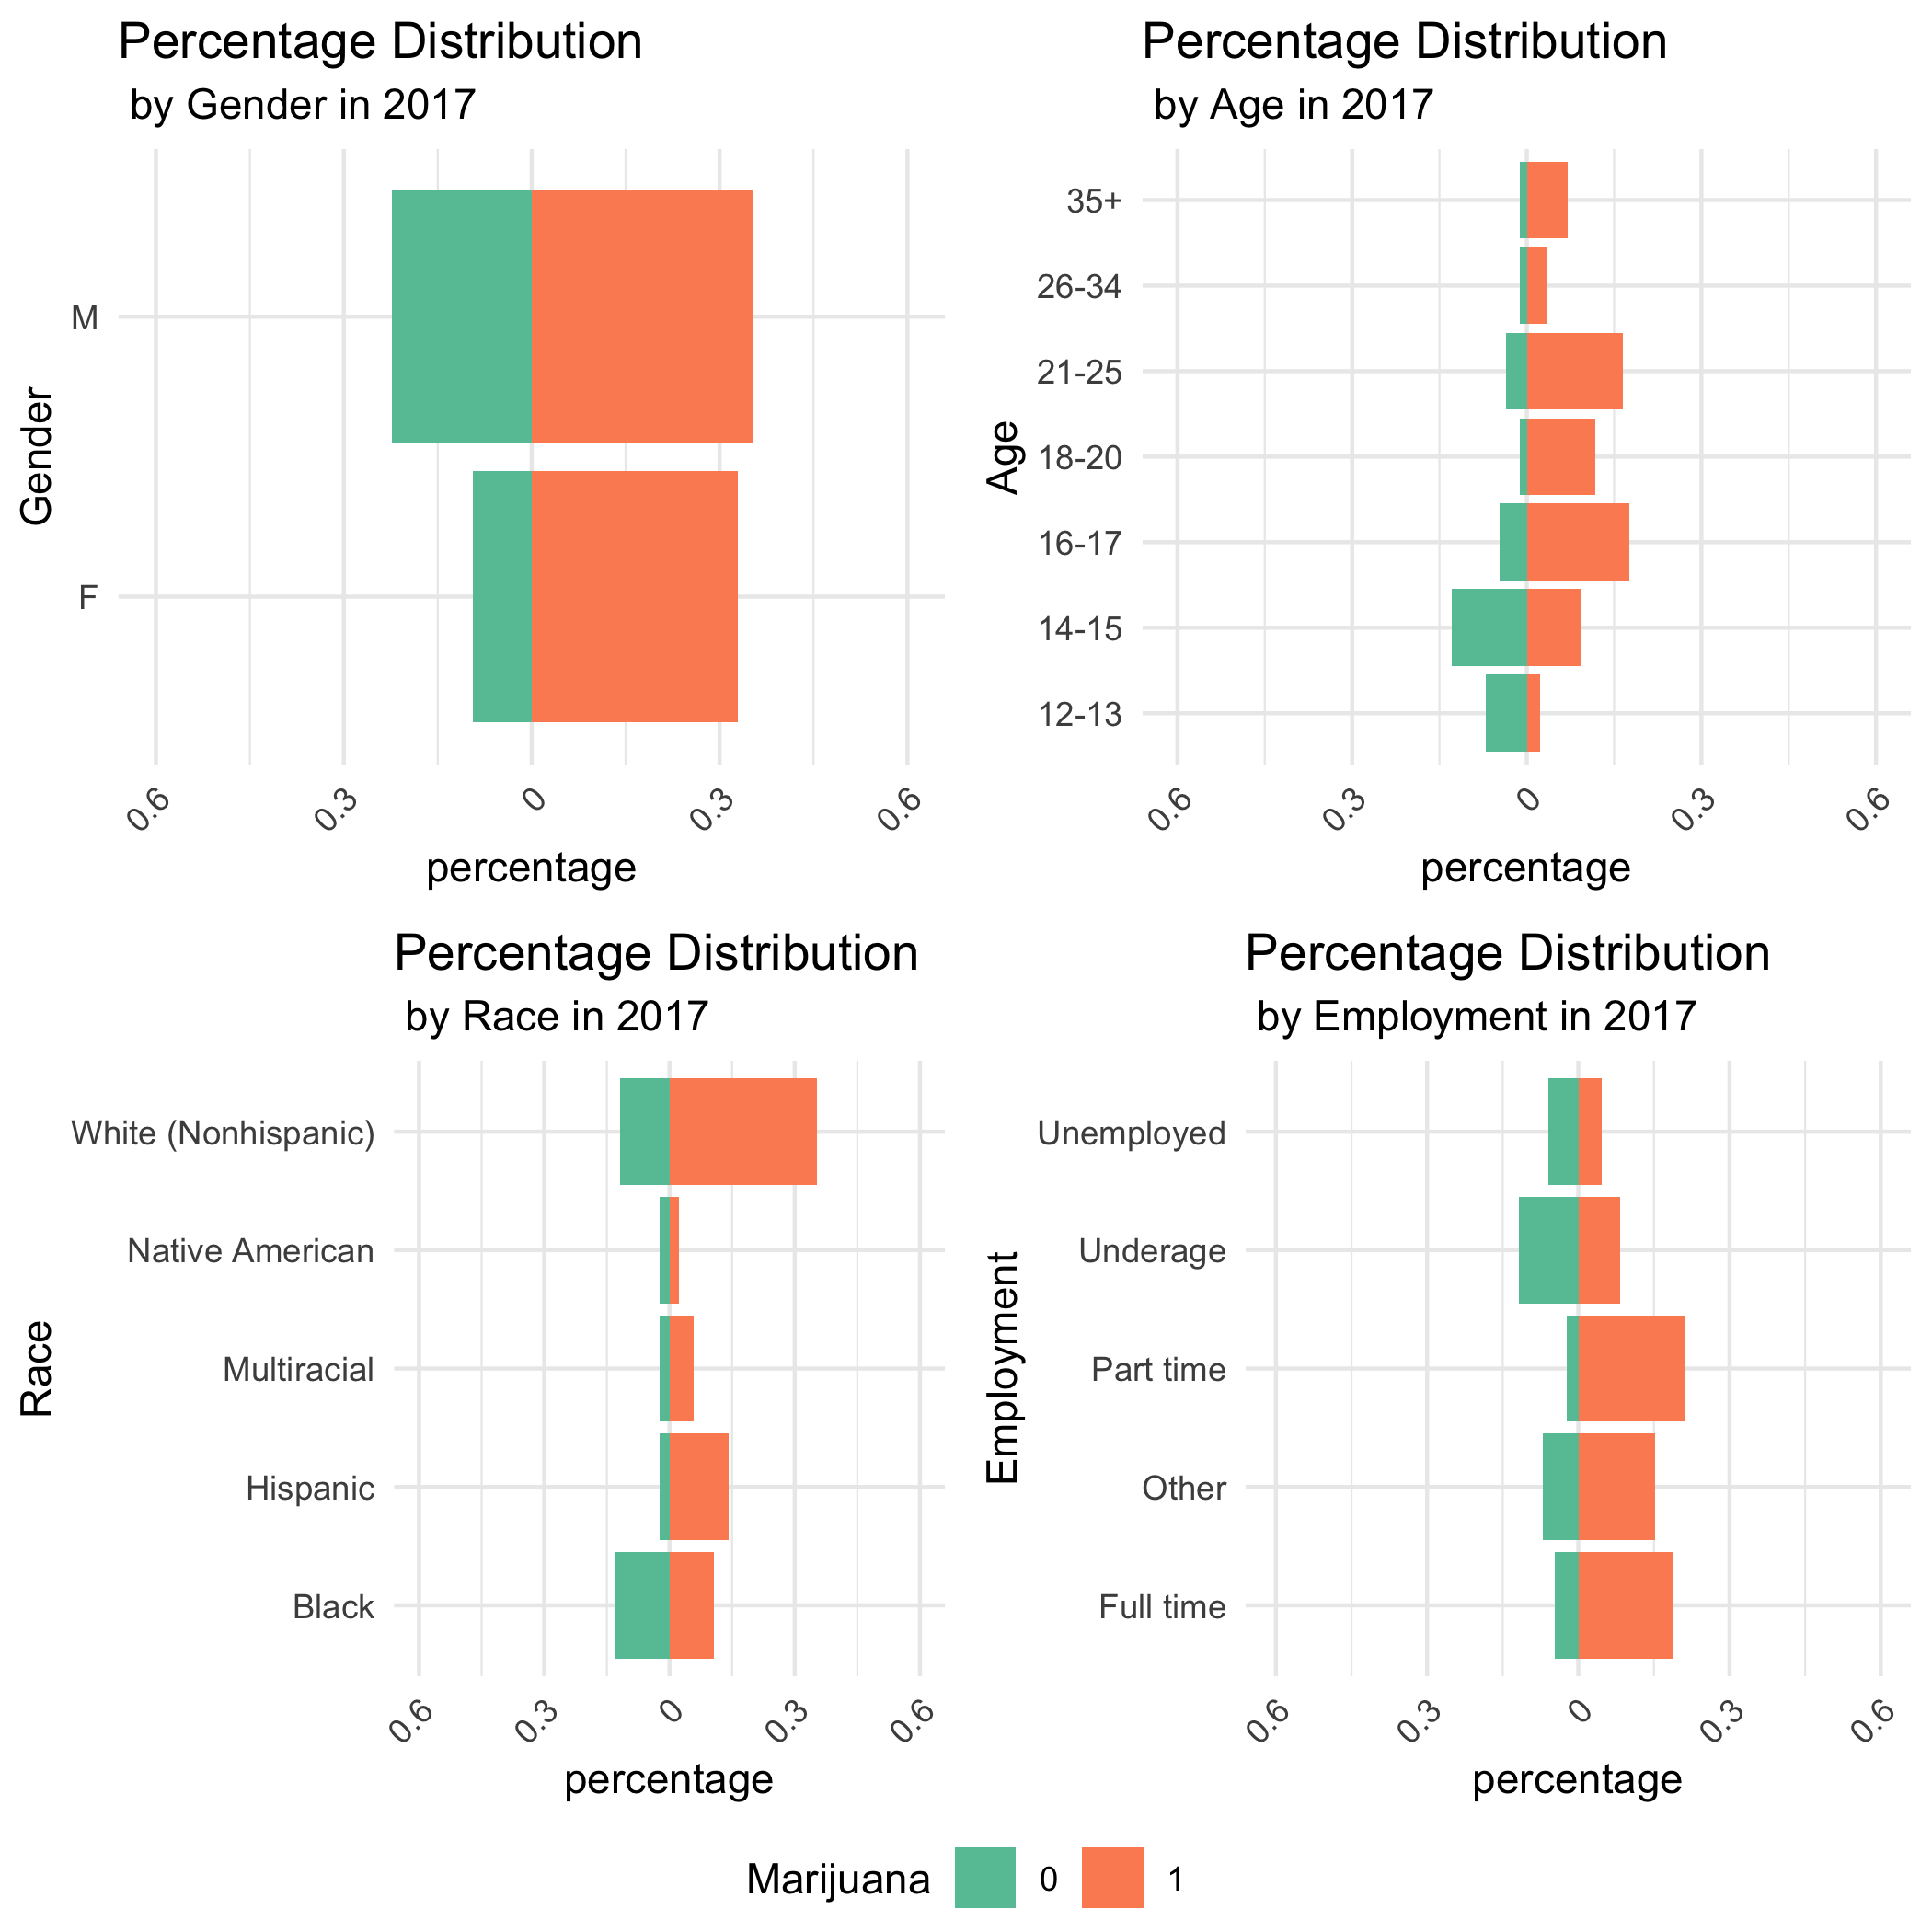
\includegraphics[scale = 0.09]{model2} \captionof{figure}{Covariate Distribution after Matching for Model 2} \end{figure} The covariate percentage distributions in Figure 4 is compared with the one in Fig. 2 for marijuana. Before matching, there appears to be a higher density of non-smokers than smokers for both genders, more for the female than male. This story changes dramatically after matching. It appears that while the proportion of smokers who are male or female is kept to similar proportions as above, the percentage of non-smokers is dropped drastically for both genders. Now males make up most of the matched sets. The distribution between control and treatment group is somewhat balanced for men but not for women. Coming along to the age distribution, the age group of $14$ to $15$ appears most matched whereas the other age groups are imbalanced in percentage. In addition, there are more smokers than non-smokers for all groups except $14$ to $15$ and $12$ to $13$. Before the age group of $35$ and up appeared balanced but after matching, it is imbalanced. The race distribution is still majorly populated by white non-hispanic people and is also imbalanced unlike before. The percentage distribution for employment appears to create balance for the unemployed and underage types where before it was imbalanced. However, the full time group of participants was balanced before matching and not after matching. 

\begin{figure}[b!] 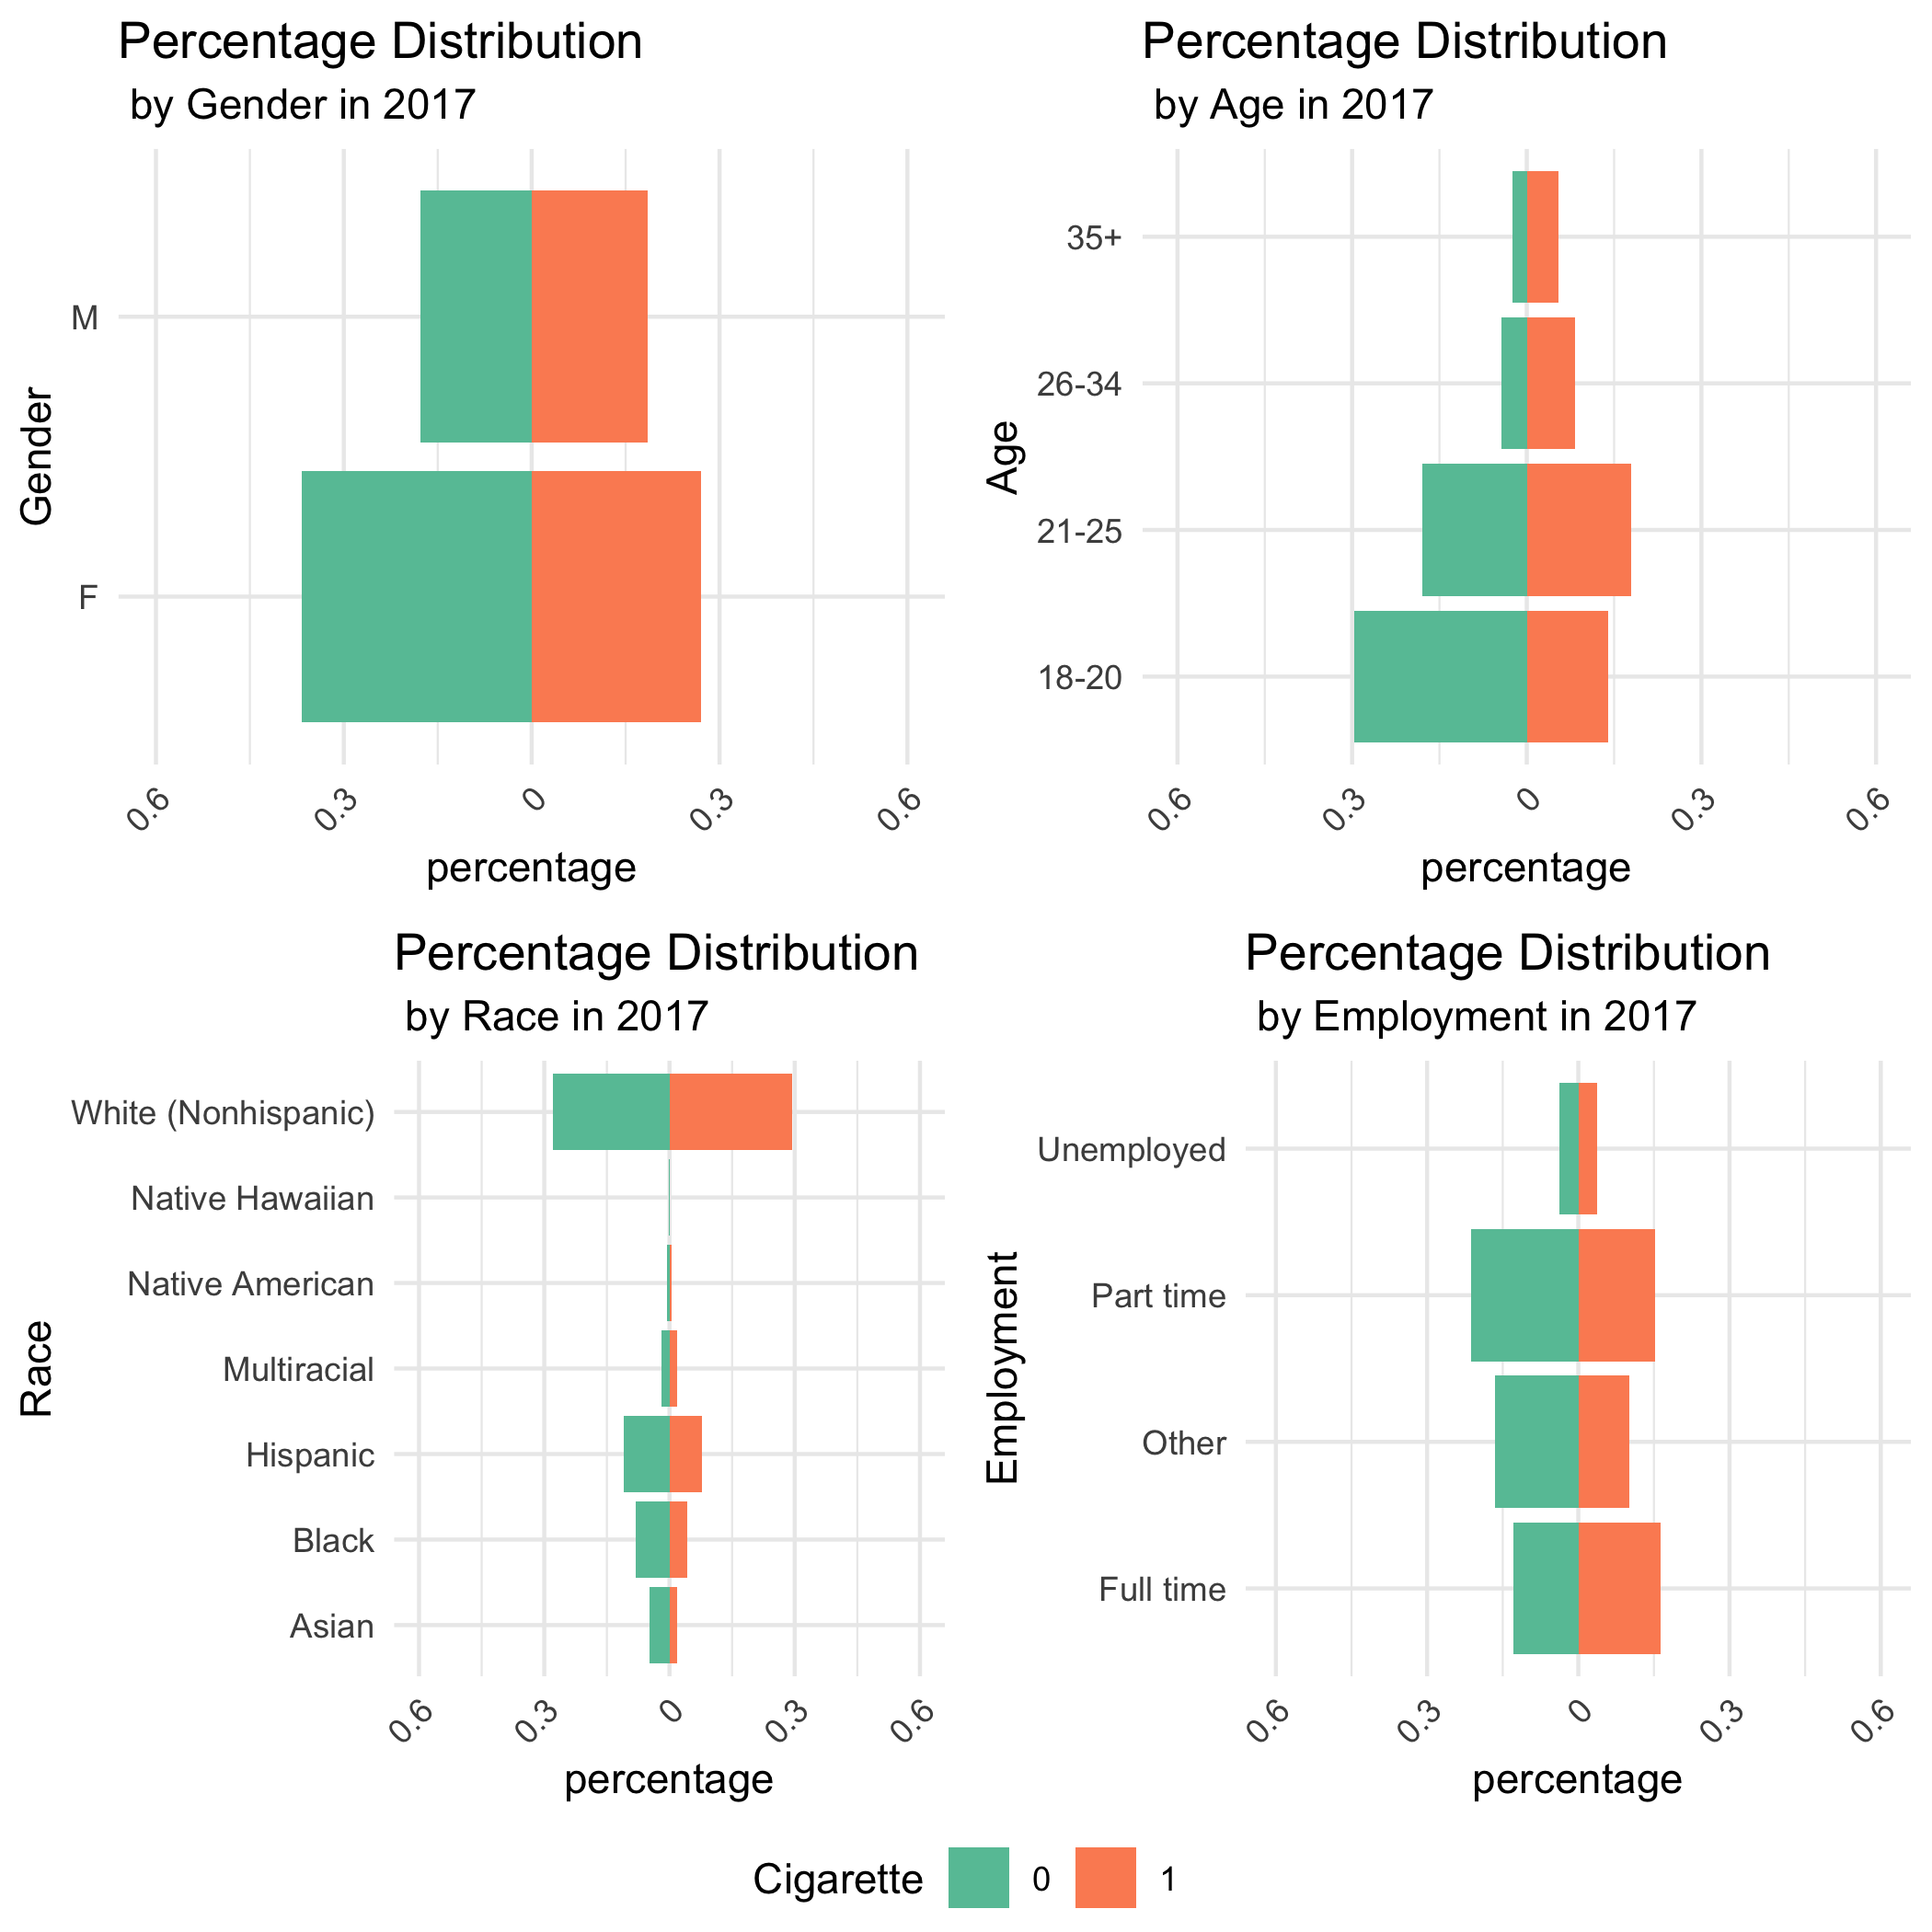
\includegraphics[scale = 0.09]{model3} \captionof{figure}{Covariate Distribution after Matching for Model 3} \end{figure}
\begin{figure}[h!] 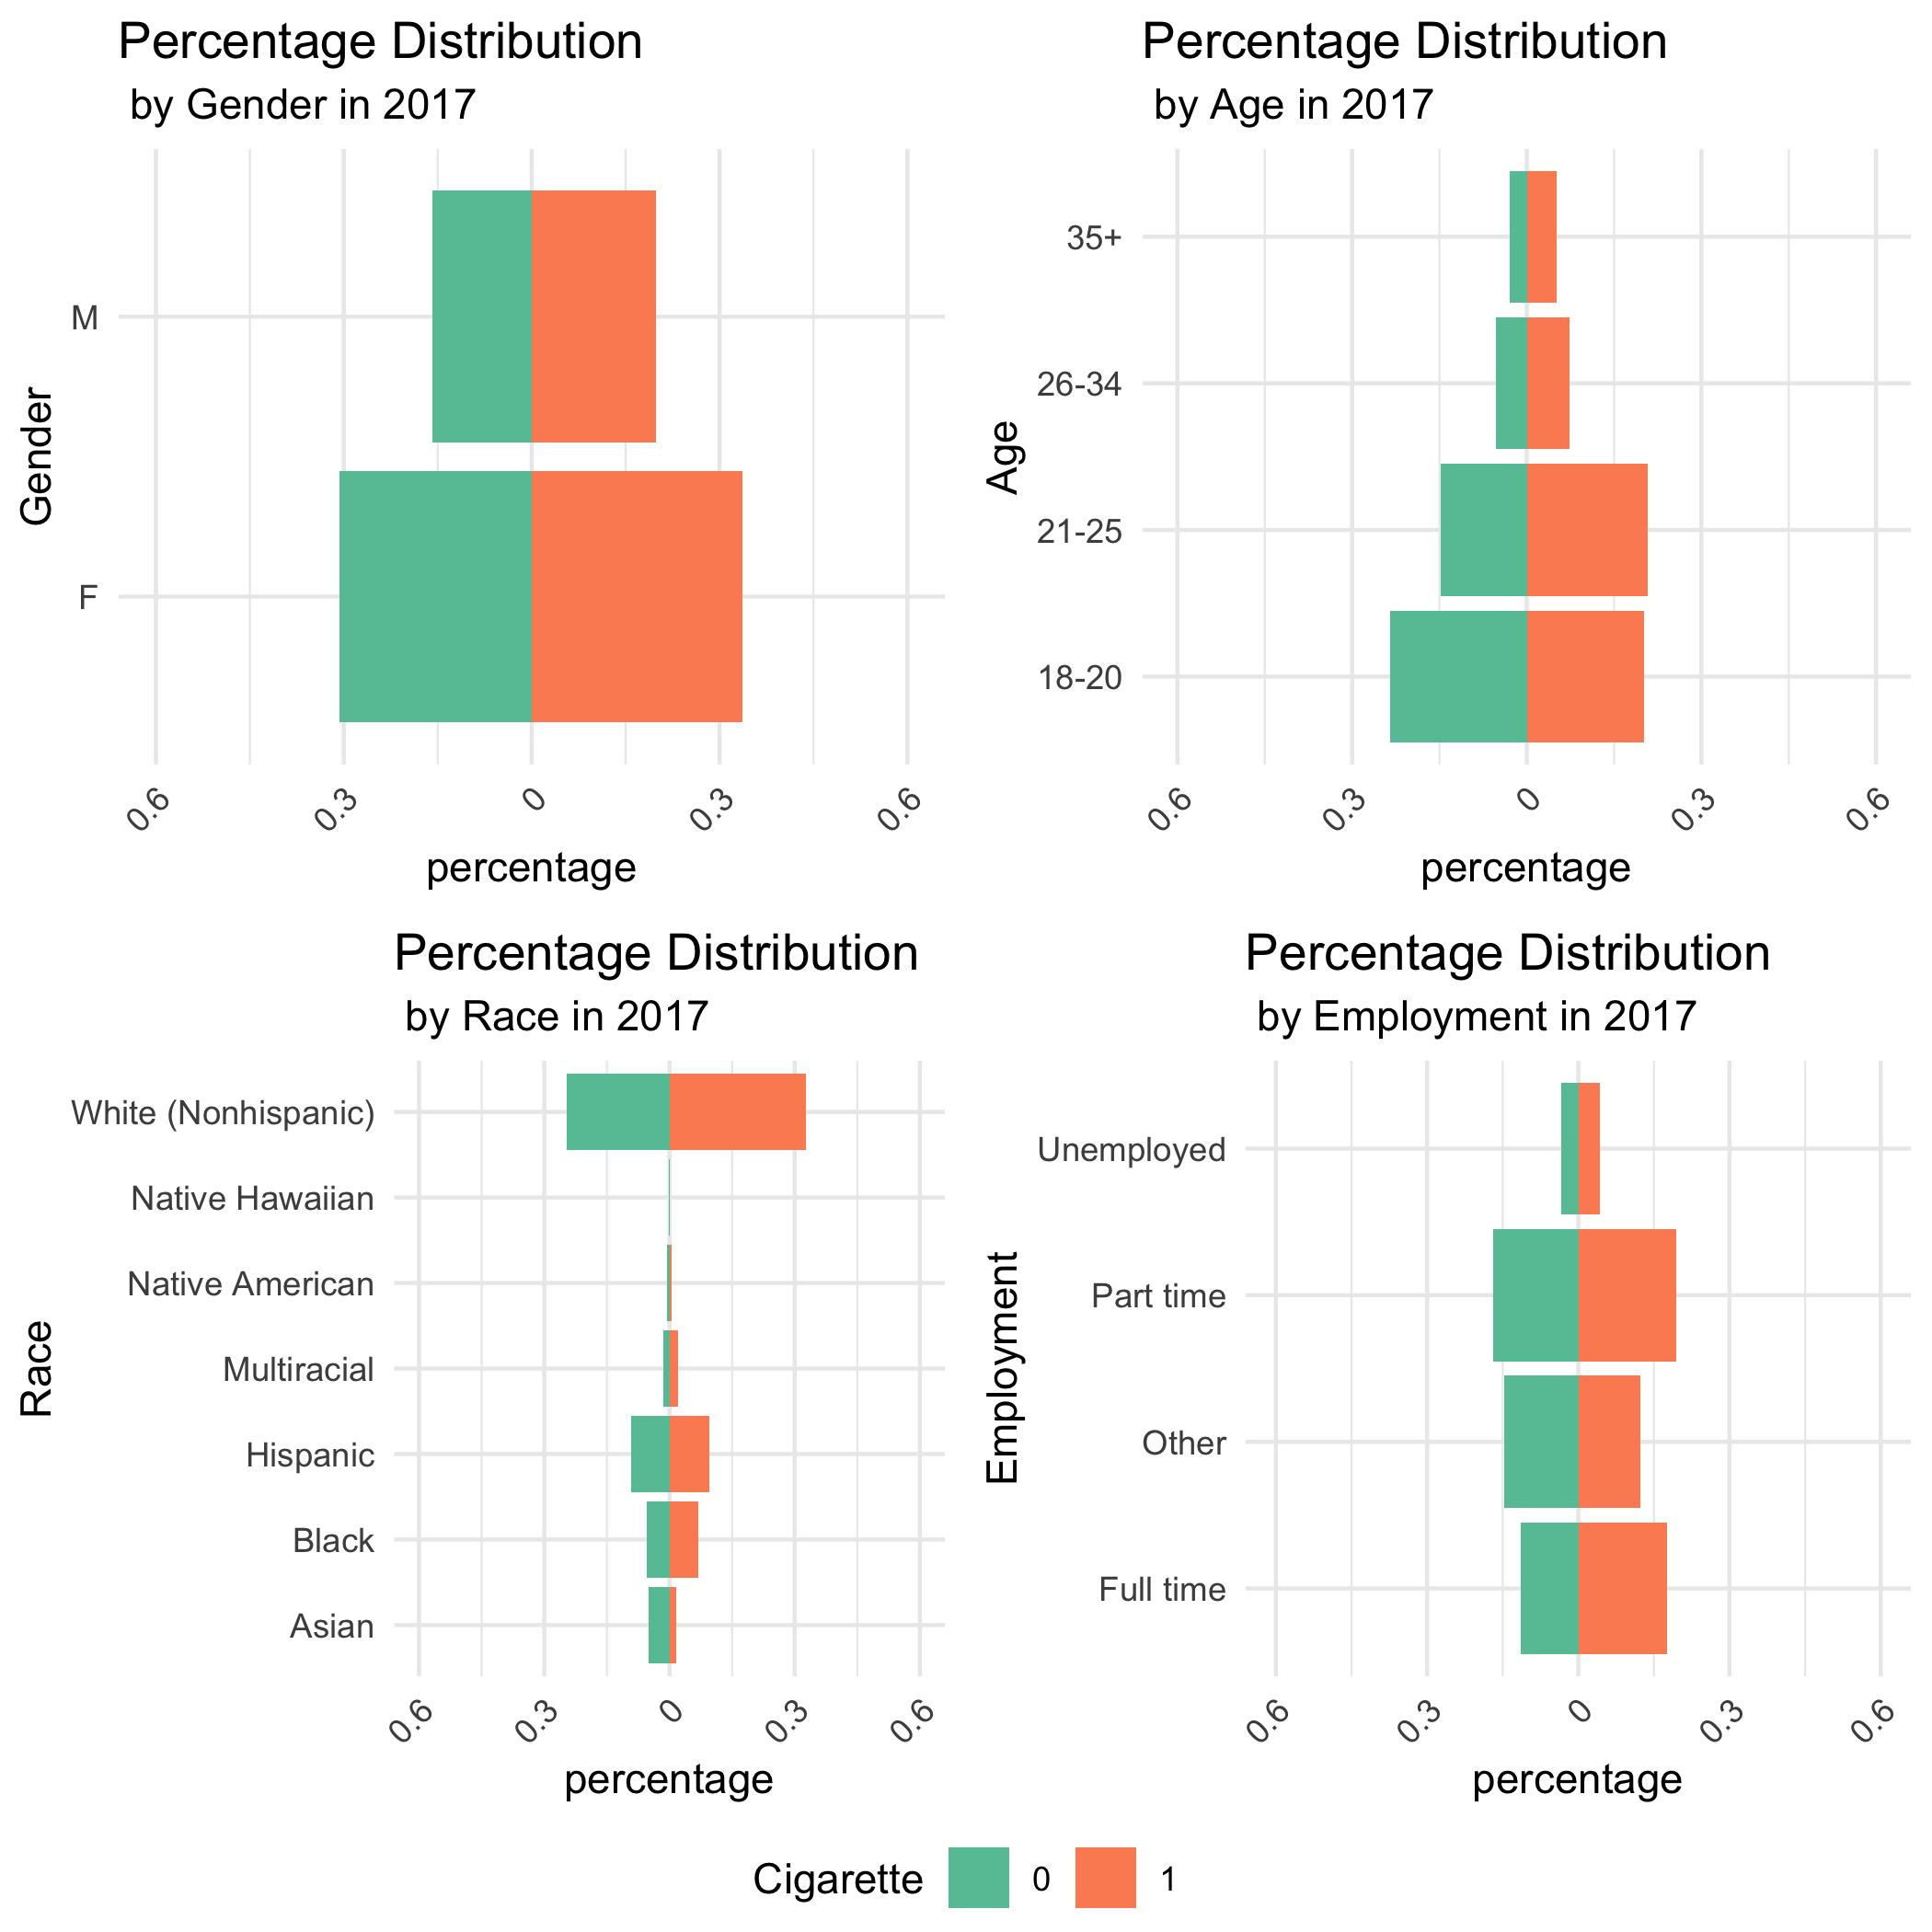
\includegraphics[scale = 0.09]{model4} \captionof{figure}{Covariate Distribution after Matching for Model 4} \end{figure}
Similar analysis can be done for the covariate distributions after matching for model 3 and 4, given in Fig. 5 and 6 respectively. In Fig. 5, the male participants are matched whereas the females are not. The $21$ to $25$ age group is matched, as well as the white non-hispanic sample and the full time employed sample. In Fig. 6, the genders are not matched, nor are the races and age groups. The age categories of $18$ to $20$ and the hispanic race group come close to being matched. Lastly, the employment is almost matched for three of the four categories. 


\section{Conclusion}

In this observational study, an attempt was made to find causal relations between taking certain drugs and criminal behaviors and emotional stress indicators using propensity score matching and logistic regression modeling. In some cases, the matching helped to find subjects that are similar to each other whereas in other, it did not do anything. By the covariate distributions after matching, it was apparent that many features such as race and age remained to be imbalanced even after using propensity score matching. Nonetheless, a few coefficients were calculated and interpreted in the context of a logistic regression framework. It was found that there's a $\approx 20\%$ percent increase in the odds of committing a burglary, arson or theft crime if one smokes cigarette, when leaving all covariates constant. Similarly, there's a $\approx 13\%$ percent increase in the odds of feeing stressed by either feeling nervousness, hopelessness or worthlessness in the past year. For marijuana use, there's a decrease in crime activity when one smokes marijuana, by $-\approx 44\%$ in the log odds of committing the crimes. Lastly, there's an increase of $\approx 65\%$ of having emotional stress if one is a marijuana user. A further investigation into the logistic regression models show that all of the $p$-value associated with these estimates are very large, signifying that the estimates are not statistically significant. 

Whether conclusions can be drawn from this study or not is debatable. Many propensity scores were not matched and in the cases they were, results were calculated to be insignificant. This study could improve by utilizing other forms of regression modeling such as doubly robust regression. To help with matching, various other forms of matching could be looked at to achieve better performance and statistically significant results. The next step in this investigation is to find out if other crimes are related to smokers, or other drug users. Effects of using hallucinogens and inhalants could be sought after. As for cigarette and marijuana, an investigation can be done to find out if these drug users try to get mental health treatment. Also, since the marijuana and emotional stress indication model gave uninterpretable results, another substitute for solving this question could be done, such as making the binary variable for stress into multivariate. This could improve solutions. Further investigation can also be done to predict if one will commit a crime or have stress in their life, using machine learning. 

\section*{Acknowledgment}

I would like to acknowledge Professor Frank Yoon, adjunct associate professor of statistics at Fordham University, for his continual effort to educate and provide feedback to students in his observational studies course, despite a low turnout.

\end{document}
